
	\section{ACM/ICPC World Finals 2013}
		\subsection{ACM/ICPC World Finals 2013 A Self-Assembly}
			\subsubsection{题目大意}
				
				
				给定 $N$ 种型号的正方形若干,各正方形的四边上均印有标志,为两个零或者一个大写字
				\begin{wrapfigure}{r}{7.0cm}
 					\centering
					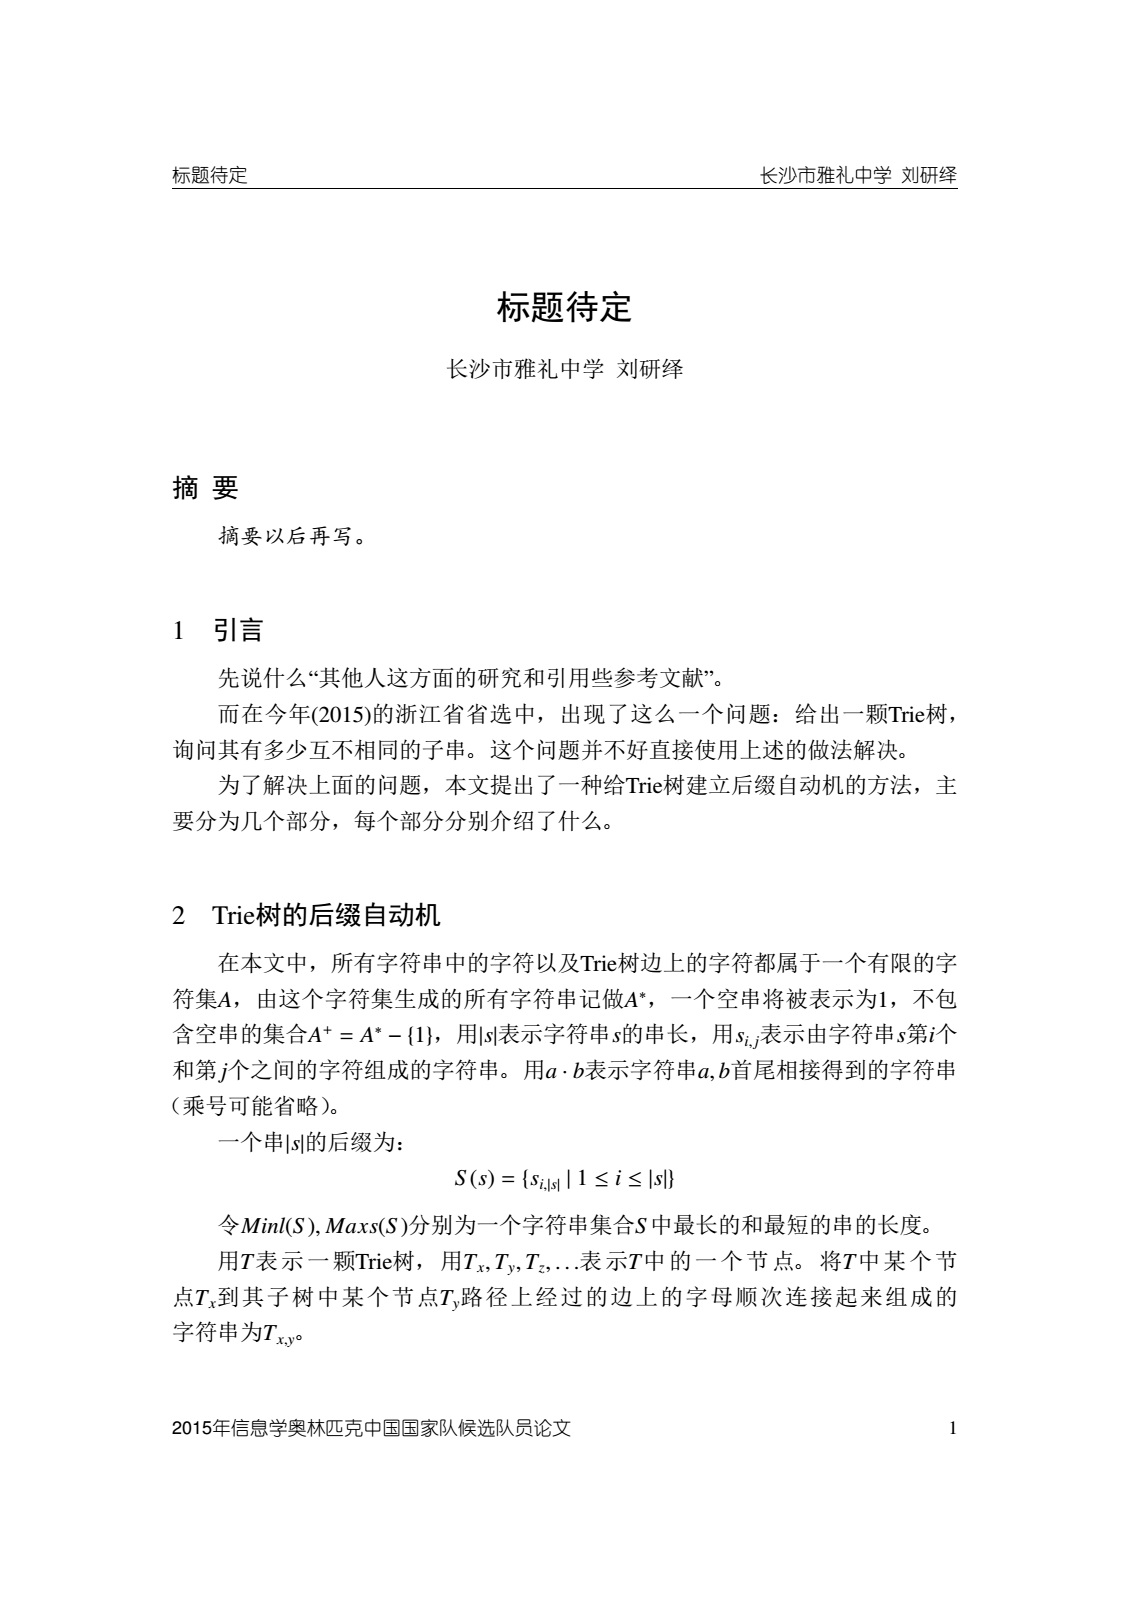
\includegraphics[width= 6.5cm]{1.jpg}
					\caption{一个例子}
				\end{wrapfigure}
				母和一个正号或负号。规定两个正
				方形能相拼当且仅当公用一条边,其均不是两个零,且字母相等,负号相反。正方形可旋转翻转,求是否存在一种拼法使得这个组合物想有多大,就能有多大。
				
				右图为一种可能的情况的拼接方案,但仅使用这些型号的正方形,只能拼出有限大小的组合物。
				
				$N \le \num{40000}$。
			
			\subsubsection{算法讨论}
				注意到,如果存在一个正方形序列链 $P_1, P_2, \ldots P_n, P_1$,两两前后拼接成链,那么可以通过翻转正方形的方式,使得这条链从左上只向右和下延伸。将翻转后的链复制任意多份,首尾拼接再按上述方式翻转,就能够构造出足够大的组合物,此时答案为是;反之,若不存在,则答案显然为否。问题即,询问是否存在这样的链。
				
				四边的标志总共有 $2 \times 26 + 1 = 53$ 种,对于每个标志可建一个对应的结点,构成图。
				对于一个四边标志为 $a,b,c,d$ 的正方形,在图上表示为 $a \rightarrow \bar{b}, a \rightarrow \bar{c}, a \rightarrow \bar{d}, b \rightarrow \bar{a}, b \rightarrow \bar{c}, \ldots, d \rightarrow \bar{c}  $ 等 $12$ 条边(两个零对应的结点不参与连边),其中 $\bar{x}$ 表示 $x$ 结点对应字母相等符号相反的结点。答案取决于是否有长度不低于 $1$ 的有向环。运行 Tarjan 算法即可求解。
			\subsubsection{时空复杂度}
				时间复杂度 $\mathcal{O}\left(|\varSigma|+N\right) = \mathcal{O}\left(N\right)$。$|\varSigma|$ 为大写字母数。
				
				空间复杂度 $\mathcal{O}\left(|\varSigma|\right) = \mathcal{O}\left(1\right)$。
		
		
		
			
		\newpage
		\subsection{ACM/ICPC World Finals 2013 C Surely You Congest}
			\subsubsection{题目大意}
				给定无向图 $G = (V,E)$。边有边权 $ W:E \mapsto \mathbb{R}_+$,表示经过该边的时间。$K$ 个人从不同的结点同时出发,欲沿最短路前往 $1$ 号结点。设计一种方案,使得不会有两个人,同时从某条道路的一端出发,同时到达另一端,且使尽可能多的人
				到达  $1$ 号结点。输出该人数。
				
				结点数 $N = |V| \le \num{25 000},$ 边数 $ M = |E| \le \num{50 000},$ 人数 $K \le \num{1 000}, \forall e \in E, $ 边权 $W(e) \le \num{10 000}$。
			\subsubsection{算法讨论}
				根据图论知识,如果边 $ e = (u,v)$  满足 $d(u) = W(e) + d(v)$,其中 $d(x)$ 表示结点 $x$ 到 $1$ 号结点的最短路长度,那么各人是有可能从 $u$ 到 $v$ 地经过这条边的;反之若  $d(u) \ne W(e) + d(v)$,则各人一定不会经过这条边。故我们可以先用堆优化的 Dijkstra 算法预处理出 $d(\cdot)$。
				
				再次使用图论知识,进一步分析可知,如两个人出发时所在结点到 $1$ 号结点的最短距离不同,那么他们一定不会产生冲突;而若两个人的出发结点到 $  1$ 号结点的最短距离相同,那么是否产生冲突就取决于是否经过了同一条边。因此我们可以对各个距离上的人分开处理。对于每一组人,则要求在两两间不经过同一条边,且均走最短路的条件下,最大化抵达 $1$ 号结点的人数。
				
				该问题可用最大流算法解决。添加一个虚拟结点 $s$,即新点集 $V^\prime = V \cup \{s\}$。对于该组所在的每一个人所在的结点 $i$, 加边 $(s,i),$容量$ f(s,i) = 1$。而对于原图中满足 $d(u) = W(e) + d(v)$ 的边 $e=(u,v)$,在网络中加
				边 $(u,v),$容量$f(u,v)=1$。设 $t = 1$ 号结点。那么网络 $\textstyle G^\prime = (V^\prime,E^\prime), E^\prime = \bigcup_{i} (s,i) \cup \bigcup_{d(u) = W(e) + d(v)} e  $ 关于容量 $f$ 的 $s-t$ 最大流就是这一组问题的答案。累加求和。
				
				在实践中,SAP 算法和 Dinic 各有优势,亦各有劣势。在这里,笔者将这两者结合起来,先使用一定时间运行 SAP 算法,若该阶段 SAP 算法出解,则累计入答案;若 SAP 算法超时,那么转用 Dinic 算法,继续计算。在该题中,该方法可以避免超时问题。
			\subsubsection{时空复杂度}
				时间复杂度 $\mathcal{O}\left(N+M \log M + K\! \cdot\! Maxflow(N,M+N)\right)$。其中 $ Maxflow(N,M))$ 表示解决 $N$ 个点, $M$ 条有向边的网络流问题的复杂度。该上限非常宽松,实际情况远远达不到该复杂度。
				
				空间复杂度 $\mathcal{O}\left(N+M\right)$。
		\newpage
		\subsection{ACM/ICPC World Finals 2013 D Factors}
			\subsubsection{题目大意}
			设 $f(x)$ 表示将整数 $x,x>1$ 唯一分解后,重新排列的方案数。例如 $f(10) = 2$ 因为 \begin{align} 10 & = 2 \cdot 5 = 5 \cdot 2 \intertext{$f(20) = 3$ 因为}  20 & = 2 \cdot 2 \cdot 5 = 2 \cdot 5 \cdot 2 = 5 \cdot 2 \cdot 2 \end{align}
			
			给定整数 $k$,求最小的 $f^{-1}(k)$,其中 $f^{-1}(x)$ 表示 $f(x)$ 的反函数
			。
			
			如最小的 $f^{-1}(1)=2,f^{-1}(2)=6,f^{-1}(3)=12,f^{-1}(105)=720$。
			
			$k < 2^{63}, $最小的 $f^{-1}(k) < 2^{63}$。多组询问。
			
			\subsubsection{算法讨论}
				由组合数学知识可知,设 $x = 2^{a_1} \cdot 3^{a_2} \cdot 5^{a_3} \cdot \cdots \cdot {p_k}^{a_k}$,其中 $p_k$ 表示第 $k$ 大的质数,则 
				\begin{align}
					f(x) = \binom{a_1 + a_2 + \cdots + a_k}{a_1, a_2, \ldots , a_k}
				\end{align}
				而如果将指数 $a_1, a_2, \ldots , a_k$ 从大到小排序为 $b_1, b_2, \ldots , b_k$,那么多项式系数 $\textstyle \binom{b_1 + b_2 + \cdots + b_k}{b_1, b_2, \ldots , b_k}$ 不会改变,即 $y = 2^{b_1} \cdot 3^{b_2} \cdot \cdots \cdot {p_k}^{b_k} \le x$ 且 $f(x) = f(y)$。故最小的 $f^{-1}(k)$ 在唯一分解后,随着质数底数的增加,指数不会上升。而满足该条件且低于 $2^{63}$ 的数非常有限,只有 \num{43607} 个,可以通过暴力搜索全部求出。找出这些数 $x$ 后,易求出其 $f(x)$ 并哈希。对于各关键字,保留最小的 $x$。最后,对于询问 $k$,在哈希表中找出答案输出即可。
			 	
				特殊处理 $f^{-1}(1)$。
			\subsubsection{时空复杂度}
				时间复杂度 $\mathcal{O}\left(g(k)\right)$。
				
				空间复杂度 $\mathcal{O}\left(g(k)\right)$。$g(k)$ 表示不超过 $k$ 且唯一分解后,随着质数底数的增加,指数不会上升的数的个数。 $g(2^{63}-1) = \num{43607}$。
			
		\newpage
		\subsection{ACM/ICPC World Finals 2013 E Harvard}
			\subsubsection{题目大意}
				有 $N$ 个内存池,各内存池有 $M$ 字节。若需访问 $1$ 号内存池里的数据,则可以直接使用 $1$ 单位的时间来完成。而若访问其他内存池中的数据,则需事先将 $BMR$ 改为该内存池的编号,再用 $1$ 单位予以访问。$BMR$ 是在其他地方存储的变量,修改其值耗费 $1$ 单位时间。
			
				现在有一个程序,包括循环语句和先后待访问的变量(变量均只有一字节),循环语句可嵌套。请合理分配该程序中的变量在内存中的位置,使得读取内存的时间最小化。
				
				变量数 $K \le \min (N\cdot M, 13), N,M \le 13$。程序源代码包含不超过 \num{1000} 个关键字(变量,循环标志)。总共要访问变量的次数不超过 \num{1e12}。
			\subsubsection{算法讨论}
				暴力搜索各变量的位置,并加以检验,取最优值。
				
				有一些有效的剪枝。
				\begin{enumerate}
					\item 分析可知,第一块内存应该尽可能的存储变量,因为其访问时间最少。先暴力搜索哪些变量进入了第一块内存池。
					\item 确定了第一块内存池中的元素后,将其从展开的程序中剔除,并统计相邻的变量各有多少。对于不在同一组内存池中的变量,其对答案的贡献值为在程序中相邻出现的次数。统计过程可用栈结构实现。
					\item 各个内存池内的元素的顺序不会影响结果,故可以规定,各内存池按从小到大的顺序搜索。
					\item 各个内存池的顺序不会影响结果,故可以规定,内存池按最大值从小到大的顺序搜索。
				\end{enumerate}
			
				设程序总共访问 $X$ 次变量。如果在枚举第一块内存池时,全部变量都进入了其中,则该情况答案为 $X$;否则,答案为 $(X + 1 + \text{剔除第一块内存后,相邻元素不在同一组的情况数})$。
			\subsubsection{时空复杂度}
				时间复杂度涉及到比较麻烦的组合数学的计算,并且上述减枝可能带来更低的上限,难以估算。但对于本题,该算法效率还算较高。
				
				空间复杂度 $\mathcal{O}\left(1\right)$。
				
		\newpage
		\subsection{ACM/ICPC World Finals 2013 F Low Power}
			\subsubsection{题目大意}
				有 $N$ 张 $2 \times K$ 的表格 $K_1,K_2, \ldots, K_N$。设 $f(A)$ 表示表格 $A$ 的第一行的最小值与第二行最小值之差的绝对值。求将 $2 N \times K$ 个数一对一的填入表格中,使得 $\textstyle \min_{i=1}^{n} f(K_i)$ 最小化。
				
				$2N \times K \le \num{1e6}$,待填入的数均为正整数,不超过 \num{1e9}。
			\subsubsection{算法讨论}
				不妨设各行最小的数从小到大排序后为 $a_1,a_2, \ldots a_{2N}$。
				\begin{theorem}
					存在一个最优解,一定是 $a_1,a_2$ 在同一个表格,$a_3,a_4$ 在同一个表格,……,$a_{2N-1},a_{2N}$ 在同一个表格。 \label{2013f1}
				\end{theorem}
				\begin{pf}
					调整法,如果当前的布局不是这样,那么必然存在 $i<j<p<q$,使得 $a_i,a_p$ 在一个表格, $a_j,a_q$ 在另一个表格。若以行为整体,调整为 $a_i,a_j$ 分一组,$a_p,a_q$ 分一组,那么两个表格的 $f$ 值都不会增加,即答案 $\textstyle \min_{i=1}^{n} f(K_i)$ 也不会增加。重复迭代上述过程,即可得到最终的布局,且该布局优于其他的任意布局。\qed
				\end{pf}
				\begin{theorem}
					存在一个最优解,同一表格中两行的最小值在即将填入的数中大小一定相邻。
				\end{theorem}
				\begin{pf}
					调整法,如果 $a_{2i-1}, a_{2i}$ 在同一个表格,且在即将填入的数字从小到大排序后形成的序列中,与 $a_{2i-1}$ 相邻的数为 $x$,其中 $x$ 在 $a_{2i-1}$ 之后,位置上异于 $a_{2i}$。根据定理  \ref{2013f1},$x$ 一定在其所在行中不是最小值,且 $a_{2i-1} \le x \le a_{2i}$。强制交换 $x$ 和 $a_{2i}$ 后,由于  $x \le a_{2i}$,故原先 $x$ 所在行的最小值不会变化,而原先 $a_{2i}$  所在行的最小值会变为 $x$,故原先 $a_{2i}$  所在的表格的 $f$ 值不会上升。反复迭代可知,大小相邻的数作为最小值不会比其他策略的值更差。\qed
				\end{pf}
				至此,可以使用二分和贪心策略解决问题。设当前猜测答案为 $K_{\text{ans}}$。那么将要填入的序列排序后扫描,若相邻的两个数相差不超过 $K_{\text{ans}}$,那么肯定可以用一张新的表格将这两个数作为最小值填入,原因是如果这样做都无解的话,那么其他填法也肯定无解,这其中有一个蕴含的关系。否则,若相邻的两个数相差大于 $K_{\text{ans}}$,则将扫描序列中最小的数填入先前的某张表格中作为较大值。如果该步骤没有空位能够容纳该值,则返回无解。若填满了 $N$ 张表格,则返回有解。使用二分算法即可在对数时间内得知答案。
			\subsubsection{时空复杂度}
				时间复杂度 $\mathcal{O}\left(N\cdot K \log M \right)$。$M$ 是待填入的数的数据规模。本题 $M = \num{1e9}$。
			
				空间复杂度 $\mathcal{O}\left(N\cdot K \right)$。
		\newpage
		\subsection{ACM/ICPC World Finals 2013 H
				Матрёшка
			}
			\subsubsection{题目大意}
				$N$ 个套娃排成一排,%大小不一,
				第 $i$ 个的大小为 $A_i$。现在要将其中一些套在一起,合并成若干个大套娃。要求
				\begin{enumerate}
					\item 整个过程只能是较大的套娃套较小的套娃。
					\item 每次只能将相邻两个套娃(可能是已经合并过的),通过打开和关闭盖子的方式将其套成(合并为)一个更大的套娃。
					\item 最终每个大套娃是由大小为 $1,2,3, \ldots, x$ 的套娃相套而成,$x$ 是大套娃所含的最小单位的套娃数。
				\end{enumerate}
				打开和关闭盖子的时间为 1。试问完成任务的最少时间。
				
				$N \le 500, 1\le  A_i \le 500,  A_i $ 为整数。
			\subsubsection{算法讨论}
				设将 $L$ 到 $R$ 的套娃套成一个单独的大套娃的时间为 $C[L][R]$,再设设处理好前 $i$ 个套娃的最少时间为 $F[i]$。那么使用时间复杂度 $\mathcal{O}\left(N^3\right)$ 的动态规划
				\begin{align}
					F[i] & = \min_{1 \le j \le i \atop \text{$j$ 到 $i$ 合并满足要求}%\{ A_j, A_{j+1}, \ldots, A_{i}\} = [1,j-i+1] \cap \mathbb{Z}
					}
					F[j-1] + C[j][i]
					\intertext{边界}
						F[0]& =0
				\end{align}
				即可求出答案 $F[N]$。下求 $C[L][R]$。
				
				同样可以使用动态规划求出,
				\begin{align}
					C[L][R] = \min_{L \le i < R}{ C[L][i] + C[i+1][R] +  W(L,i,R)}
				\end{align}
				其中 $W(L,i,R)$ 表示合并好 $L$ 到 $i$ 以及 $(i+1)$ 到 $R$ 的套娃后,仅合并这两者的最少所需时间。设 $k$ 为最小值较小的一堆套娃中,尺寸低于
				另一堆
				最小值的套娃数,那么 $W(L,i,R) = R-L+1-k$。
				忽略 $W(\cdot,\cdot,\cdot)$ 	 的计算时间,该动态规划的时间复杂度%为
				  $\mathcal{O}\left(N^3\right)$ 。
				
				而 $W(\cdot,\cdot,\cdot)$ 也
				可以用均摊 $\mathcal{O}\left(1\right)$ 时间求出。不失一般性,设 $L$ 到 $i$ 尺寸的最小值相对较大,为 $MinValue$,另一种情况对称处理。不妨动态维护 $(i+1)$ 到 $R$ 的套娃中,各个尺寸 $x$ 的套娃数 $H[x]$。对于每个 $i$ 的遍历值,$H\left(\cdot\right)$只需修改一个数,可以均摊 $\mathcal{O}\left(1\right)$ 算出。而 $\textstyle W(L,i,R) = \sum_{j=1}^{MinValue-1} H[j]$。根据 $MinValue$ 与 $A[i]$ 的关系,若 $MinValue>A[i]$ 则 $ W $函数的值较原来自减一,否则保持原样,也可以在 $\mathcal{O}\left(1\right)$ 时间维护好 $W(L,i,R)$。
				另一方面,$i$ 从 $L$ 枚举到 $(R - 1)$ 的过程中,前者的最小值  $MinValue$ 也会发生变化,且不断地减小。若  $MinValue$ 从 $x$ 减少到 $(x -1)$,那么 $W$ 函数较原来会自减 $H[x-1]$。$MinValue$ 的值只可能从 $(R-L+1)$ 减少到 $1$,减少次数不会超过  $(R-L+1)$ ,故也可以在均摊 $\mathcal{O}\left(1\right)$ 时间维护好 $W(L,i,R)$。
				综上,整个算法的时间复杂度可控制在 $\mathcal{O}\left(N^3\right)$ 。
			\subsubsection{时空复杂度}
				时间复杂度 $\mathcal{O}\left(N^3\right)$。
				
				空间复杂度 $\mathcal{O}\left(N^2\right)$。
			
		\newpage
		\subsection{ACM/ICPC World Finals 2013 I Pirate Chest}
			\subsubsection{题目大意}
				在 $N \times M$ 的网格状池塘里放入底部尺寸不超过 $P \times Q$ 的箱子,高度任意,但放入后其顶部的高度必须严格低于水面,并且长宽高为整数,与网格对齐。任意一个网格内池塘的底部平齐,深度由 $N \times M$ 的深度矩阵 $A$ 给出。 
				试最大化箱子的体积。
				
				$N,M \le 500, A_{i,j} \le \num{1e9}, A_{i,j}$ 为非负整数。
			\subsubsection{算法讨论}
				不妨先考虑一个一维版本的问题,即  $N = 1$ 的情况。假设箱子跨过了 $(1,i)$ 的格子,且它是所有被覆盖的格子中,深度最浅的。那么箱子的
				高度 $h$ 应当满足
				\begin{align}
					h& < \frac{Sh}{N \times M} + A_{i,j}
					\intertext{即}
					h &< \frac{A_{i,j}\times N \times M}{N \times M - S}\\
					h &= \left\lceil{(A_{i,j} \times N \times M)} / {(N \times M - S)} \right\rceil -1 \label{Piratecalc}
				\end{align}	
				其中 $S$ 为箱子底部的真实表面积。而箱子体积 $V = Sh$,由此可见,$S$ 应当尽可能的大。
				
				可以使用单调栈预处理出 $l_i$,表示最大的 $j, j<i$ 使得 $A_{1,j}<A_{1,i}$,以及 $r_i$,最小的 $j, j> i$ 使得 $A_{1,j}<A_{1,i}$。那么所有满足 $(1,i)$ 为被覆盖的格子中,深度最浅的摆放方法中,最大的底面积为 $S = \min( r_i - l_i -1 ,Q)$。代入 \eqref{Piratecalc} 即可求得高度 $h$ 和 体积 $V$。该子问题时间复杂度 $\mathcal{O}\left(M\right)$。
				
				对于原问题,不妨枚举箱子所跨的行,再合并成一行,使用上述的方法求得最大体积,取最优值,就可以求得答案。
				注意到 $P \times  Q$ 的尺寸可以旋转,故还需交换 $P, Q$ 的值再计算一次。
				仅枚举跨越的行复杂度为 $\mathcal{O}\left(N \cdot M\right)$。
				
			\subsubsection{时空复杂度}
				时间复杂度 $\mathcal{O}\left(N\cdot M^2\right)$。
					
				空间复杂度 $\mathcal{O}\left(N\cdot M\right)$。\newpage
		\subsection{ACM/ICPC World Finals 2013 J Pollution Solution}
			\subsubsection{题目大意}
				求半圆
				\begin{align}
					R: x^2+y^2 \le r^2 \land y>0
				\end{align}
				与简单多边形交的面积。
				
				简单多边形的点数 $N \le 100$,且总在 $x$ 轴上方。
			
			\subsubsection{算法讨论}
				如图 \ref{convert},求多边形面积时,我们可以转化为求 $N$ 个有向三角形的面积之和。此题也可借鉴该思想。
				\begin{figure}[!htb]
				\centering
				\begin{tikzpicture}[shorten >=1pt,node distance=2cm,on grid,>=stealth',thick,
					every state/.style={fill,draw=none,orange,text=white!80!orange,circular drop shadow},
					accepting/.style ={green!50!black,text=green!50!black!20!white},
					initial/.style ={red,text=white!80!red},scale= 0.25 ]
					\definecolor{qqzzcc}{rgb}{0,0.6,0.8}
					\definecolor{ffdxqq}{rgb}{1,0.84,0}
					\definecolor{zzwwff}{rgb}{0.6,0.4,1}
					\definecolor{ffttww}{rgb}{1,0.2,0.4}
					\definecolor{ffzzzz}{rgb}{1,0.6,0.6}
					\definecolor{ffzztt}{rgb}{1,0.6,0.2}
					
					\draw[->] (-11,0) -- (11,0) node[right] {$x$};	
					\draw[->] (0,-1) -- (0,11) node[right] {$y$};
					\foreach \x in {-10,-5,5,10}
					\draw[shift={(\x,0)},color=black] (0pt,10pt) -- (0pt,-10pt) node[below] {\footnotesize $\x$};		
					\draw[color=black] (0pt,-40pt) node[left] {\footnotesize $0$};
					\foreach \y in {5,10}
						\draw[shift={(0,\y)},color=black] (10pt,0pt) -- (-10pt,0pt) node[left] {\footnotesize $\y$};
%					\draw[dashed] (0,0) -- (2,0);
%					\draw[dashed] (0,1) -- (2,1);
%					\draw[dashed] (0,2) -- (2,2);
%					\draw[dashed] (0,0) -- (0,2);
%					\draw[dashed] (1,0) -- (1,2);
%					\draw[dashed] (2,0) -- (2,2);
					\draw[draw = zzwwff,dashed, fill = none,smooth,domain=0:180,opacity = 0.45] (10,0) -- plot({10*cos(\x)},{10*sin(\x)}) -- cycle;
					
					\draw[draw = none, fill = ffzztt,smooth,domain=0:90,opacity = 0.45] (8,2) --
						(8,14) --
						(0,14) --
						(0,6) --
						(-8,14) --
						(-8,2) -- cycle;

					\draw[->,color=ffzztt, fill = none,domain=-90:205]  plot({4+2*cos(\x+45)},{8+2*sin(\x+45)}) ;
					
										
%					\draw[draw = none, fill = qqzzcc,smooth,domain=0:90,opacity = 0.45] (0,0) -- (1,0) -- plot({2-cos(\x)},{sin(\x)})  -- (2,2) -- (1,2) --  plot({cos(\x)},{2-sin(\x)}) -- cycle;
					
%					\draw[line width=1pt,smooth,domain=0:90] plot({cos(\x)},{2-sin(\x)});
%					\draw[line width=1pt,smooth,domain=0:90] plot({2-cos(\x)},{sin(\x)});
					\draw[->] (12,5.5) -- (18,5.5);
					\begin{scope}[xshift=30 cm]
					
					\draw[->] (-11,0) -- (11,0) node[right] {$x$};	
					\draw[->] (0,-1) -- (0,11) node[right] {$y$};
					\foreach \x in {-10,-5,5,10}
					\draw[shift={(\x,0)},color=black] (0pt,10pt) -- (0pt,-10pt) node[below] {\footnotesize $\x$};		
					\draw[color=black] (0pt,-40pt) node[left] {\footnotesize $0$};
					\foreach \y in {5,10}
						\draw[shift={(0,\y)},color=black] (10pt,0pt) -- (-10pt,0pt) node[left] {\footnotesize $\y$};
%					\draw[dashed] (0,0) -- (2,0);
%					\draw[dashed] (0,1) -- (2,1);
%					\draw[dashed] (0,2) -- (2,2);
%					\draw[dashed] (0,0) -- (0,2);
%					\draw[dashed] (1,0) -- (1,2);
%					\draw[dashed] (2,0) -- (2,2);
					\draw[draw = zzwwff,dashed, fill = none,smooth,domain=0:180,opacity = 0.45] (10,0) -- plot({10*cos(\x)},{10*sin(\x)}) -- cycle;
					\draw[draw = ffdxqq, fill = ffdxqq!60!white,smooth,domain=0:90,fill opacity = 0.45] 
						(0,0) -- (8,2) --  (8,14) -- cycle;
					\draw[color = ffdxqq,->, domain=-90:205]  plot({6+1.5*cos(\x)},{4.5+1.5*sin(\x)}) ;
					
					\draw[draw = ffdxqq, fill = ffdxqq!60!white,smooth,domain=0:90,fill opacity = 0.45] 
						(0,0) -- (8,14) -- (0,14) -- cycle;
					\draw[color = ffdxqq,->, domain=-90:205]  plot({3+1.5*cos(\x+38)},{11.5+1.5*sin(\x+38)}) ;
					
					\draw[draw = ffdxqq, fill = ffdxqq!60!white,smooth,domain=0:90,fill opacity = 0.45] 
						(0,0) -- (0,14) --  (0,6) -- cycle;

					\draw[draw = ffdxqq, fill = ffdxqq!60!white,smooth,domain=0:90,fill opacity = 0.45] 
						(0,0) -- (0,6) --  (-8,14) -- cycle;
					\draw[color = ffdxqq,->, domain=-90:205]  plot({-2+1*cos(\x+52)},{6+1*sin(\x+52)}) ;
					\draw[draw = ffdxqq, fill = ffdxqq!60!white,smooth,domain=0:90,fill opacity = 0.45] 
						(0,0) -- (-8,14) --  (-8,2) -- cycle;
					\draw[color = ffdxqq,->, domain=-90:205]  plot({-6+1.5*cos(\x+41)},{4.5+1.5*sin(\x+41)}) ;
					\draw[draw = qqzzcc, fill = qqzzcc!60!white,smooth,domain=0:90,fill opacity = 0.45] 
						(0,0) -- (-8,2) --  (8,2)  -- cycle;
					\draw[color = qqzzcc,->, domain=-90:205]  plot({1.5*1.65*cos(-\x-62)},{1.15+0.5*sin(-\x-62)}) ;
										
%					\draw[draw = none, fill = qqzzcc,smooth,domain=0:90,opacity = 0.45] (0,0) -- (1,0) -- plot({2-cos(\x)},{sin(\x)})  -- (2,2) -- (1,2) --  plot({cos(\x)},{2-sin(\x)}) -- cycle;
					
%					\draw[line width=1pt,smooth,domain=0:90] plot({cos(\x)},{2-sin(\x)});
%					\draw[line width=1pt,smooth,domain=0:90] plot({2-cos(\x)},{sin(\x)});
					
					
					\end{scope}
				\end{tikzpicture}
			\caption{ 转为有向三角形(黄正蓝负) } \label{convert}
			\vspace{-1em}
			\end{figure}
			
			如图 \ref{add},先求出各线段与圆的交点。方法是将每一段线段写为参数方程 $\mathbf{p} = \mathbf{a} + \mathbf{v}t , 0 \le t \le 1$,代入圆方程 $\mathbf{p}^2 = r^2$,解关于参数 $t$ 的一元二次方程$(\mathbf{a} + \mathbf{v}t)^2 = r^2$,代回参数方程求得交点。再将这些交点插入到多边形顶点序列中。这样做的好处是,多边形的本质未改变,而相邻点间的线段要么全部位于圆内,要么全部位于圆外。而具体是在圆内还是圆外,可通过线段中点到原点的距离与半径的关系来判断。
			
			
			\begin{figure}[!htb]
				\centering
				\begin{tikzpicture}[shorten >=1pt,node distance=2cm,on grid,>=stealth',thick,
					every state/.style={fill,draw=none,orange,text=white!80!orange,circular drop shadow},
					accepting/.style ={green!50!black,text=green!50!black!20!white},
					initial/.style ={red,text=white!80!red},scale= 0.25 ]
					\definecolor{qqzzcc}{rgb}{0,0.6,0.8}
					\definecolor{ffdxqq}{rgb}{1,0.84,0}
					\definecolor{zzwwff}{rgb}{0.6,0.4,1}
					\definecolor{ffttww}{rgb}{1,0.2,0.4}
					\definecolor{ffzzzz}{rgb}{1,0.6,0.6}
					\definecolor{ffzztt}{rgb}{1,0.6,0.2}
					
					\draw[->] (-11,0) -- (11,0) node[right] {$x$};	
					\draw[->] (0,-1) -- (0,11) node[right] {$y$};
					\foreach \x in {-10,-5,5,10}
					\draw[shift={(\x,0)},color=black] (0pt,10pt) -- (0pt,-10pt) node[below] {\footnotesize $\x$};		
					\draw[color=black] (0pt,-40pt) node[left] {\footnotesize $0$};
					\foreach \y in {5,10}
						\draw[shift={(0,\y)},color=black] (10pt,0pt) -- (-10pt,0pt) node[left] {\footnotesize $\y$};
%					\draw[dashed] (0,0) -- (2,0);
%					\draw[dashed] (0,1) -- (2,1);
%					\draw[dashed] (0,2) -- (2,2);
%					\draw[dashed] (0,0) -- (0,2);
%					\draw[dashed] (1,0) -- (1,2);
%					\draw[dashed] (2,0) -- (2,2);
					\draw[draw = zzwwff,dashed, fill = none,smooth,domain=0:180,opacity = 0.45] (10,0) -- plot({10*cos(\x)},{10*sin(\x)}) -- cycle;
					
					\draw[draw = none, fill = ffzztt,smooth,domain=0:90,opacity = 0.45] (8,2) --
						(8,14) --
						(0,14) --
						(0,6) --
						(-8,14) --
						(-8,2) -- cycle;
										
%					\draw[draw = none, fill = qqzzcc,smooth,domain=0:90,opacity = 0.45] (0,0) -- (1,0) -- plot({2-cos(\x)},{sin(\x)})  -- (2,2) -- (1,2) --  plot({cos(\x)},{2-sin(\x)}) -- cycle;
					
%					\draw[line width=1pt,smooth,domain=0:90] plot({cos(\x)},{2-sin(\x)});
%					\draw[line width=1pt,smooth,domain=0:90] plot({2-cos(\x)},{sin(\x)});
					\draw[->] (12,5.5) -- (18,5.5);
					
					
					\draw[fill=ffzztt!80!black,draw=none] (8,2) circle (0.25cm)
										(8,14) circle (0.25cm)
										(0,14) circle (0.25cm)
										(0,6) circle (0.25cm)
										(-8,14) circle (0.25cm)
										(-8,2) circle (0.25cm);
					\begin{scope}[xshift=30 cm]
					
					\draw[->] (-11,0) -- (11,0) node[right] {$x$};	
					\draw[->] (0,-1) -- (0,11) node[right] {$y$};
					\foreach \x in {-10,-5,5,10}
					\draw[shift={(\x,0)},color=black] (0pt,10pt) -- (0pt,-10pt) node[below] {\footnotesize $\x$};		
					\draw[color=black] (0pt,-40pt) node[left] {\footnotesize $0$};
					\foreach \y in {5,10}
						\draw[shift={(0,\y)},color=black] (10pt,0pt) -- (-10pt,0pt) node[left] {\footnotesize $\y$};
%					\draw[dashed] (0,0) -- (2,0);
%					\draw[dashed] (0,1) -- (2,1);
%					\draw[dashed] (0,2) -- (2,2);
%					\draw[dashed] (0,0) -- (0,2);
%					\draw[dashed] (1,0) -- (1,2);
%					\draw[dashed] (2,0) -- (2,2);
					\draw[draw = zzwwff,dashed, fill = none,smooth,domain=0:180,opacity = 0.45] (10,0) -- plot({10*cos(\x)},{10*sin(\x)}) -- cycle;
					
					\draw[draw = none, fill = ffzztt,smooth,domain=0:90,opacity = 0.45] (8,2) --
						(8,14) --
						(0,14) --
						(0,6) --
						(-8,14) --
						(-8,2) -- cycle;
					
					\draw[fill=ffzztt!80!black,draw=none] (8,2) circle (0.25cm)
										(8,14) circle (0.25cm)
										(0,14) circle (0.25cm)
										(0,6) circle (0.25cm)
										(-8,14) circle (0.25cm)
										(-8,2) circle (0.25cm)
										(-8,6) circle (0.25cm)
										(8,6) circle (0.25cm)
										(0,10) circle (0.25cm)
										(-3.403124,9.403124) circle (0.25cm);
										
										
%					\draw[draw = none, fill = qqzzcc,smooth,domain=0:90,opacity = 0.45] (0,0) -- (1,0) -- plot({2-cos(\x)},{sin(\x)})  -- (2,2) -- (1,2) --  plot({cos(\x)},{2-sin(\x)}) -- cycle;
					
%					\draw[line width=1pt,smooth,domain=0:90] plot({cos(\x)},{2-sin(\x)});
%					\draw[line width=1pt,smooth,domain=0:90] plot({2-cos(\x)},{sin(\x)});
					
					
					\end{scope}
				\end{tikzpicture}
			\caption{ 求交点,加点 } \label{add}
			\vspace{-1em}
			\end{figure}
				
			对于在圆内的部分,其对交面积的贡献为前后端点$(x_1,y_1),(x_2,y_2)$ 的叉积的一半 
			\begin{align}
				\frac{1}{2}(x_1,y_1) \times (x_2,y_2) = \frac{1}{2}x_1y_2-\frac{1}{2}x_2y_1
			\end{align}
			而在圆外的部分,对交面积的贡献实质为一个扇形的面积,有向圆心角的大小
			\begin{align}
				|\theta| = \arccos \frac{(x_1,y_1)  \cdot (x_2,y_2)}{\left|(x_1,y_1)\right|\!\!\, \cdot\!\!\, \left|(x_2,y_2)\right|}
						=  \arccos \frac{x_1x_2+y_1y_2}{\sqrt{\left(x_1^2+y_1^2\right)\!\!\, \cdot\!\!\, \left(x_2^2+y_2^2\right)}}
			\end{align}
			而其正负性与 $\left((x_1,y_1) \times (x_2,y_2)\right)$ 相同。代入扇形面积公式 $ \textstyle S = \frac{1}{2} \theta r^2$ 即为该线段对交面积的贡献。求和。
			\begin{figure}[!htb]
				\centering
				\begin{tikzpicture}[shorten >=1pt,node distance=2cm,on grid,>=stealth',thick,
					every state/.style={fill,draw=none,orange,text=white!80!orange,circular drop shadow},
					accepting/.style ={green!50!black,text=green!50!black!20!white},
					initial/.style ={red,text=white!80!red},scale= 0.25 ]
					\definecolor{qqzzcc}{rgb}{0,0.6,0.8}
					\definecolor{ffdxqq}{rgb}{1,0.84,0}
					\definecolor{zzwwff}{rgb}{0.6,0.4,1}
					\definecolor{ffttww}{rgb}{1,0.2,0.4}
					\definecolor{ffzzzz}{rgb}{1,0.6,0.6}
					\definecolor{ffzztt}{rgb}{1,0.6,0.2}
					
					\draw[->] (-11,0) -- (11,0) node[right] {$x$};	
					\draw[->] (0,-1) -- (0,11) node[right] {$y$};
					\foreach \x in {-10,-5,5,10}
					\draw[shift={(\x,0)},color=black] (0pt,10pt) -- (0pt,-10pt) node[below] {\footnotesize $\x$};		
					\draw[color=black] (0pt,-40pt) node[left] {\footnotesize $0$};
					\foreach \y in {5,10}
						\draw[shift={(0,\y)},color=black] (10pt,0pt) -- (-10pt,0pt) node[left] {\footnotesize $\y$};
%					\draw[dashed] (0,0) -- (2,0);
%					\draw[dashed] (0,1) -- (2,1);
%					\draw[dashed] (0,2) -- (2,2);
%					\draw[dashed] (0,0) -- (0,2);
%					\draw[dashed] (1,0) -- (1,2);
%					\draw[dashed] (2,0) -- (2,2);
					\draw[draw = zzwwff,dashed, fill = none,smooth,domain=0:180,opacity = 0.45] (10,0) -- plot({10*cos(\x)},{10*sin(\x)}) -- cycle;
					
					\draw[draw = none, fill = ffdxqq!60!white,smooth,domain=0:90,opacity = 0.45] (0,0) --
						(6,2) --
						(2,8) -- cycle;
					\draw[color = ffdxqq!70!white, ->, dashed] (0,0) -- (6,2);
					\draw[color = ffdxqq!70!white, ->,dashed] (0,0) -- (2,8);
					\draw[color = ffdxqq, ->] (6,2) -- (2,8);
										
%					\draw[draw = none, fill = qqzzcc,smooth,domain=0:90,opacity = 0.45] (0,0) -- (1,0) -- plot({2-cos(\x)},{sin(\x)})  -- (2,2) -- (1,2) --  plot({cos(\x)},{2-sin(\x)}) -- cycle;
					
%					\draw[line width=1pt,smooth,domain=0:90] plot({cos(\x)},{2-sin(\x)});
%					\draw[line width=1pt,smooth,domain=0:90] plot({2-cos(\x)},{sin(\x)});
%					\draw[->] (12,5.5) -- (18,5.5);
					
					
					\begin{scope}[xshift= 28cm]
					
					\draw[->] (-11,0) -- (11,0) node[right] {$x$};	
					\draw[->] (0,-1) -- (0,11) node[right] {$y$};
					\foreach \x in {-10,-5,5,10}
					\draw[shift={(\x,0)},color=black] (0pt,10pt) -- (0pt,-10pt) node[below] {\footnotesize $\x$};		
					\draw[color=black] (0pt,-40pt) node[left] {\footnotesize $0$};
					\foreach \y in {5,10}
						\draw[shift={(0,\y)},color=black] (10pt,0pt) -- (-10pt,0pt) node[left] {\footnotesize $\y$};
%					\draw[dashed] (0,0) -- (2,0);
%					\draw[dashed] (0,1) -- (2,1);
%					\draw[dashed] (0,2) -- (2,2);
%					\draw[dashed] (0,0) -- (0,2);
%					\draw[dashed] (1,0) -- (1,2);
%					\draw[dashed] (2,0) -- (2,2);
					\draw[draw = zzwwff,dashed, fill = none,smooth,domain=0:180,opacity = 0.45] (10,0) -- plot({10*cos(\x)},{10*sin(\x)}) -- cycle;
					
%					\draw[draw = none, fill = ffdxqq!60!white,smooth,domain=0:90,opacity = 0.45] (0,0) --
%						(12,2) --
%						(3,14) -- cycle;
					
					\draw[color = qqzzcc!70!white, ->, dashed] (0,0) -- (12,2);
					\draw[color = qqzzcc!70!white, ->,dashed] (0,0) -- (3,14);
					\draw[color = qqzzcc, ->] (3,14) -- (12,2);
					
					\draw[draw = none, fill = qqzzcc!60!white,smooth,domain=9.462322208025617391140070541742:77.905242922987898747566331385281,opacity = 0.45] (0,0) --
						plot({10*cos(\x)},{10*sin(\x)})
						-- cycle;
					
					\draw[color = qqzzcc, -> ,domain=77.905242922987898747566331385281:9.462322208025617391140070541742] 
						plot({3*cos(\x)},{3*sin(\x)});
					\node[color = qqzzcc] at ({4*cos(43.683782565506758069353200963511)},{4*sin(43.683782565506758069353200963511)}) {$\theta$};
					
%					\draw[draw = none, fill = qqzzcc,smooth,domain=0:90,opacity = 0.45] (0,0) -- (1,0) -- plot({2-cos(\x)},{sin(\x)})  -- (2,2) -- (1,2) --  plot({cos(\x)},{2-sin(\x)}) -- cycle;
					
%					\draw[line width=1pt,smooth,domain=0:90] plot({cos(\x)},{2-sin(\x)});
%					\draw[line width=1pt,smooth,domain=0:90] plot({2-cos(\x)},{sin(\x)});
					
					
					\end{scope}
				\end{tikzpicture}
			\caption{ 两种情况对面积的贡献} 
			\vspace{-1em}
			\end{figure}
			
			\subsubsection{时空复杂度}
				时间复杂度 $\mathcal{O}\left(N\right)$。
				
				空间复杂度 $\mathcal{O}\left(1\right)$。
		\newpage
		\subsection{ACM/ICPC World Finals 2013 K Up a Tree}
			\subsubsection{题目大意}
			在以下三段有问题的代码中
			\begin{multicols}{3}
				\begin{algorithm}[H]
				\caption{前序遍历}
				\label{}
					\begin{algorithmic}[1]
						\Function{Pre}{$x$}
							\State \Call{Print}{$x$}
							\State \Call{\fbox{ 甲 }}{$x$ 的左儿子}
							\State \Call{\fbox{ 乙 }}{$x$ 的右儿子}
						\EndFunction
					\end{algorithmic}
				\end{algorithm}
				\begin{algorithm}[H]
				\caption{中序遍历}
				\label{}
					\begin{algorithmic}[1]
						\Function{In}{$x$}
							\State \Call{\fbox{ 丙 }}{$x$ 的左儿子}
							\State \Call{Print}{$x$}
							\State \Call{\fbox{ 丁 }}{$x$ 的右儿子}
						\EndFunction
					\end{algorithmic}
				\end{algorithm}
				\begin{algorithm}[H]
				\caption{后序遍历}
				\label{}
					\begin{algorithmic}[1]
						\Function{Post}{$x$}
							\State \Call{\fbox{ 戊 }}{$x$ 的左儿子}
							\State \Call{\fbox{ 己 }}{$x$ 的右儿子}
							\State \Call{Print}{$x$}
						\EndFunction
					\end{algorithmic}
				\end{algorithm}
			\end{multicols}
			填入恰好两个 \Call{Pre}{} 恰好两个 \Call{In}{} 和恰好两个\Call{Post}{},使得存在一个树,分别调用这三个函数后,得到的先序中序后序遍历为给定的串,并使得输入的树的正确前序中序后序遍历的字典序最小化。
			
			$4 \le \text{给定串的长度} \le 26$。
			\subsubsection{算法讨论}
			填写源代码的情况数只有 $\textstyle \binom{6}{2,2,2} = 90$ 种,可先枚举。
			
			这样,问题简化为,固定代码,给定一个二叉树调用\Call{Pre}{}, \Call{In}{} 和 \Call{Post}{} 函数中某几个的输出,求字典序最小的树使其满足条件。
			
			不妨递归处理,枚举左儿和右儿的元素数量,就可以确定根以及左右儿调用\Call{Pre}{}, \Call{In}{} 和 \Call{Post}{} 某几个后的输出,且规模更小。继续分治处理即可。最后合并答案,选择一个字典序最小的树返回。边界条件为输出全部为空串,此时可直接返回空树。
			
			有一些有效的剪枝。
			\begin{enumerate}
				\item 对于同一棵树,若几个函数输出的长度不一,可直接返回无解。
				\item 对于同一棵树,若有结点在某些函数的输出中出现,而在另一些函数的输出中未出现,可直接返回无解。
				\item 在递归调用时,若对于一棵子树,运行相同的函数,得出的输出序列不同,可直接返回无解。
				\item 枚举左右儿元素数后,若输出序列确定的根不一,可直接跳过此次枚举。
				\item 若左右儿对应的子问题有一个无解,可直接跳过此次枚举。
				\item 记忆化搜索
			\end{enumerate}
%			可加快搜索效率。
			\subsubsection{时空复杂度}
				时间复杂度 $\mathcal{O}\left(N^5\right)$,使用这些减枝后,实际运行时间远远达不到这个上限。
					
				空间复杂度 $\mathcal{O}\left(N^4\right)$。使用压位,索引,垃圾回收等方式可以进一步减少空间占用。
		\newpage